%-----------------------------------------------------------------------------%
\chapter{\babTiga}
%-----------------------------------------------------------------------------%
Pada bab ini dipaparkan mengenai rancangan dan tahap-tahap proses ekstraksi relasi semantik, mulai dari rancangan pengembangan korpus, pembentukan \textit{seed}, pembentukan \textit{pattern}, ekstraksi \textit{pair}, \textit{cycle semi-supervised}, dan strategi evaluasi yang dilakukan untuk pasangan kata relasi Bahasa Indonesia. 


%-----------------------------------------------------------------------------%
\section{Spesifikasi Penelitian}
%-----------------------------------------------------------------------------%
Berikut adalah spesifikasi penelitian yang dilaksanakan dan batas-batasanya.
\begin{itemize}
  \item Relasi yang diperhatikan adalah \textit{hypernym-hyponym}.
  \item Kelas kata yang diperhatikan adalah \textit{noun} dan \textit{proper noun}.
  \item Kata yang diekstrak termasuk \textit{multi word}. Contoh: sepak bola, Amerika Serikat, dan lainnya.
\end{itemize}

\begin{figure}
    \centering
    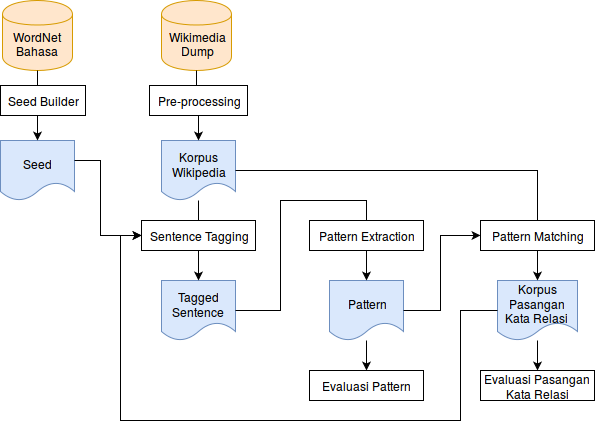
\includegraphics[width=\linewidth]{pics/Pic01-SemiSupervisedCycle}
    \caption{Arsitektur Penelititan}
    \label{fig:arsitektur-penelitian}
\end{figure}
%-----------------------------------------------------------------------------%
\section{Rancangan Pengembangan Korpus}
%-----------------------------------------------------------------------------%
Pengembangan korpus pasangan kata berelasi yang digunakan pada penelitian ini menggunakan arsitektur yang dapat dilihat pada gambar \ref{fig:arsitektur-penelitian}. Terdapat dua sumber data utama yang digunakan yaitu WordNet Bahasa untuk pembentukan \textit{seed} dan artikel Wikipedia Bahasa Indonesia sebagai korpus teks. Secara garis besar, terdapat enam tahap yang perlu dilakukan yaitu pembuatan \textit{seed}, \textit{pre-processing} data Wikipedia, \textit{sentence tagging}, \textit{pattern extraction}, \textit{pattern matching}, dan terakhir adalah evaluasi. Untuk proses \textit{sentence tagging}, \textit{pattern extraction}, dan \textit{pattern matching} dilakukan secara berulang, sesuai dengan metode \textit{bootstrapping}. Berikut adalah penjelasan singkat setiap tahapan.
\begin{enumerate}
  \item Pembentukan \textit{seed} dilakukan untuk mendapatkan pasangan kata berelasi yang digunakan sebagai dasar penelitian. Proses ini memanfaatkan \textit{resource} yang dimiliki WordNet Bahasa.
  \item Artikel Wikipedia diperoleh dalam bentuk \textit{Wikipedia dump} dan perlu diolah sehingga memiliki representasi sesuai dengan format yang diharapkan. Informasi yang diperlukan hanya bagian isi artikel dan kemudian ditulis berdasarkan kalimat untuk setiap baris.
  \item Menggunakan \textit{seed} dan korpus Wikipedia, dilakukan \textit{tagging} pasangan kata berelasi terhadap kalimat-kalimat yang ada. Kalimat yang mengandung pasangan kata berelasi akan ditandai dan disimpan sebagai dasar proses selanjutnya.
  \item Kalimat-kalimat yang sudah di-\textit{tag} dengan pasangan kata berelasi kemudian akan digunakan untuk proses \textit{pattern extraction}. Hasil dari proses ini adalah sejumlah \textit{pattern} leksikal terbaik dari banyak \textit{pattern} unik yang dihasilkan.
  \item Proses berikutnya adalah \textit{pattern matching} dimana \textit{pattern} hasil ekstraksi dan korpus Wikipedia kembali digunakan untuk membentuk pasangan kata relasi baru (\textit{pair}).
  \item Korpus pasangan relasi kata yang terbentuk digunakan untuk iterasi selanjutnya sesuai dengan metode \textit{bootstrapping}. Proses iterasi dilakukan hingga pasangan kata relasi baru yang dihasilkan jenuh. Terakhir dilakukan evaluasi untuk mengetahui akurasi data yang dihasilkan.
\end{enumerate}

Proses ini diharapkan dapat menghasilkan korpus pasangan kata relasi \textit{hyponym-hypernym} yang berkualitas baik dan berukuran besar. \textit{Pair} yang dihasilkan ditulis dalam bentuk \textit{tuple} $(kata_hyponym;kata_hypernym)$ dengan kedua kata berada dalam kelas kata benda.


%-----------------------------------------------------------------------------%
\section{Pre-processing Data}
%-----------------------------------------------------------------------------%
Proses inti dari penelitian ini, \textit{pattern extraction} dan \textit{matching}, memerlukan dua masukan utama yaitu sejumlah pasangan kata \textit{hypernym-hyponym} dan teks dokumen yang digunakan sebagai korpus. Pasangan kata \textit{hypernym-hyponym} digunakan untuk proses pembentukan \textit{pattern} sementara teks dokumen digunakan untuk memperoleh pasangan kata baru. Dikarenakan belum ada korpus pasangan kata relasi \textit{hypernym-hyponym} Bahasa Indonesia, perlu didefinisikan \textit{seed} yang akan digunakan sebagai dasar pasangan kata \textit{hypernym-hyponym}. Teks dokumen yang digunakan, yaitu Wikipedia, juga memerlukan pemrosesan sebelum menjadi masukan sistem.

%-----------------------------------------------------------------------------%
\subsection{Pre-processing Data Wikipedia}
%-----------------------------------------------------------------------------%
Data Wikipedia yang diperoleh dari Wikimedia \textit{dumps} masih mengandung banyak \textit{tag} yang tidak digunakan pada penelitian ini seperti \textit{tag} \textit{id} dan \textit{revision}. Selain itu simbol-simbol khusus (\textit{markup}). Penelitian ini ingin mengekstrak \textit{pattern} dari \textit{free text}, sehingga format-format khusus tersebut perlu dibersihkan. Setelah data Wikipedia dibersihkan dari simbol-simbol tersebut, langkah selanjutnya adalah merepresentasikan korpus dalam bentuk kalimat. 

Artikel-artikel Wikipedia dibentuk ke dalam format yang telah didefinisikan dengan satu kalimat dipisahkan untuk setiap barisnya. Data tersebut juga digunakan untuk proses \textit{part-of-speech tagging}. Hasil dari \textit{pre-processing} data Wikipedia adalah dua korpus besar yaitu korpus tanpa \textit{pos tag} yang digunakan sebagai masukan \textit{pattern extraction} dan korpus dengan \textit{pos tag} yang digunakan sebagai masukan \textit{pattern matching}. 

%-----------------------------------------------------------------------------%
\subsection{Pengumpulan Seed}
%-----------------------------------------------------------------------------%
Pasangan kata relasi \textit{hypernym-hyponym} diambil dari data yang dimilki oleh WordNet Bahasa yang dikembangkan oleh NTU. Pemanfaatan WordNet Bahasa dilatarbelakangi jumlahnya yang lebih besar dibanding Indonesian WordNet (IWN). Relasi semantik antar kata pada WordNet Bahasa memanfaatkan WordNet Princeton versi 3.0. \textit{Synset} pada WordNet Bahasa dipetakan ke \textit{synset} WordNet Princeton, sehingga relasi semantik yang dimiliki oleh WordNet Princeton ikut diwarisi. Alasan lain penggunaan WordNet Bahasa adalah karena telah terintegrasi dengan \textit{tools} nltk sehingga dapat langsung digunakan untuk membentuk \textit{seed} secara mudah.

Seluruh lema Bahasa Indonesia yang dimiliki oleh WordNet tersebut akan dipasangkan dengan lema \textit{hypernym}-nya, sehingga terbentuk relasi biner antara kata yang merupakan \textit{hyponym} dan kata yang merupakan \textit{hypernym}. Format untuk korpus ini mengikut format korpus pasangan kata relasi yang akan digunakan.


%-----------------------------------------------------------------------------%
\section{Pembentukan Pattern}
%-----------------------------------------------------------------------------%
\textit{Pattern} leksikal yang akan digunakan ingin seluruhnya dibentuk secara otomatis oleh sistem. Terdapat dua masukan utama untuk proses ini yaitu pasangan kata relasi \textit{hypernym-hyponym} yang telah diketahui dan korpus dokumen. Pada tahap awal, pasangan kata relasi masukan adalah \textit{seed} yang dibentuk menggunakan WordNet Bahasa. Untuk tahap selanjutnya, pasangan kata relasi menggunakan korpus \textit{pair} hasil proses ekstraksi. Terdapat dua tahapan utama dalam pembentukan \textit{pattern} yaitu \textit{sentence tagging} dan \textit{pattern extraction}.

%-----------------------------------------------------------------------------%
\subsection{Sentence Tagging}
%-----------------------------------------------------------------------------%
\textit{Sentence tagging} adalah proses \textit{intermediate} sebelum sistem dapat membentuk sebuah \textit{pattern} leksikal. Proses ini akan memberi \textit{tag hypernym} dan \textit{hyponym} terhadap suatu kata di dalam kalimat. Masukan untuk proses ini adalah pasangan kata relasi dan korpus Wikipedia tanpa \textit{pos tag}. Untuk setiap kalimat dalam korpus Wikipedia, dicek apakah kalimat tersebut mengandung pasangan kata relasi. Jika mengandung, maka kata dalam kalimat yang merupakan pasangan kata akan di-\textit{tag} \textit{hypernym} dan \textit{hyponym}. Satu kalimat dicocokan dengan seluruh pasangan kata relasi karena terdapat kasus dimana satu kalimat mengandung lebih dari satu pasangan kata relasi. Proses ini menghasilkan kalimat-kalimat Wikipedia yang telah diberi \textit{tag hypernym} atau \textit{hyponym}.

%-----------------------------------------------------------------------------%
\subsection{Pattern Extraction}
%-----------------------------------------------------------------------------%
Setelah didapatkan kumpulan kalimat yang sudah diberi \textit{tag hypernym} dan \textit{hyponym}, dicari barisan kata yang mirip dan dapat dijadikan sebuah \textit{pattern}. \textit{Pattern extraction} adalah proses untuk mendapatkan \textit{pattern} leksikal yang kemunculannya sering dalam korpus. Masukan dari proses ini adalah kalimat-kalimat Wikipedia yang telah diberi \textit{tag hypernym} dan \textit{hyponym}. Proses ini akan menghasilkan kumpulan \textit{pattern} unik yang terurut berdasarkan bobotnya. Dari \textit{pattern} unik tersebut, akan diambil sejumlah \textit{pattern} terbaik untuk kemudian digunakan sebagai dasar pembentukan \textit{pair} baru.


%-----------------------------------------------------------------------------%
\section{Ekstraksi Pair}
%-----------------------------------------------------------------------------%
Tujuan utama dari penelitian ini adalah membentuk korpus pasangan kata relasi, sehingga proses ekstraksi \textit{pair} adalah tahapan utama dalam keseluruhan penelitian. Pada proses ini, dimanfaatkan \textit{pattern} yang telah terbentuk sebelumnya untuk mengekstrak pasangan kata baru. Pasangan kata tersebut kemudian difilter sebelum digabung ke dalam korpus pasangan kata relasi.

%-----------------------------------------------------------------------------%
\subsection{Pattern Matching}
%-----------------------------------------------------------------------------%
\textit{Pattern matching} adalah proses mencocokan suatu \textit{pattern} ke dalam teks dokumen. Proses ini dilaksanakan untuk mendapatkan pasangan kata relasi (\textit{pair}) baru. Dua masukan utama untuk proses ini adalah pattern dan korpus Wikipedia \textit{pos tag}. Penggunaan korpus Wikipedia dengan \textit{pos tag} untuk membatasi \textit{pair} yang terekestrak hanya berasal dari kelas kata \textit{noun} atau \textit{proper noun}. Namun, tidak seluruh \textit{pair} yang dihasilkan benar memiliki relasi \textit{hypernym-hyponym}. Untuk itu, dihitung nilai bobot untuk seluruh \textit{pair} yang dihasilkan. Nilai bobot digunakan untuk dibandingkan dengan nilai threshold yang didefinisikan. Hanya \textit{pair} yang bobotnya melebihi nilai \textit{threshold} yang dapat masuk ke korpus pasangan kata relasi.


%-----------------------------------------------------------------------------%
\section{Cycle Semi-Supervised}
%-----------------------------------------------------------------------------%
Pembelajaran menggunakan pendekatan \textit{semi supervised learning} dilatarbelakangi ketersediaan pasangan kata relasi semantik yang telah diketahui (\textit{seed}) berukuran terbatas dan korpus berukuran besar yang belum dianotasi. Ingin didapatkan \textit{pair} baru dari korpus yang belum diantoasi tersebut. Metode \textit{semi supervised} yang diterapkan adalah \textit{Bootstrapping}. Untuk lebih spesifiknya, algoritma \textit{bootstrapping} yang digunakan adalah \textit{Basilisk} dengan beberapa modifikasi. Pemilihan \textit{Basilisk} sebagai metode \textit{Bootrapping} didasari proses ekstraksi \textit{seed} baru yang memanfaatkan \textit{pattern}. Pada penelitian ini, dilakukan modifikasi sesuai kebutuhan. Secara umum, proses \textit{bootstrapping} dikelompokan ke dalam dua tahap yaitu iterasi ke-1 dan iterasik ke-2 hingga n.

Penggunaan \textit{seed} yang berasal dari WordNet Bahasa hanya dilakukan pada iterasi pertama. Pada iterasi ini, \textit{pattern} yang merupakan hasil dari \textit{seed} dengan lema sama dan \textit{seed strict} digabung dan diurutkan berdasarkan bobot \textit{pattern}. Lima \textit{pattern} terbaik diambil untuk selanjutnya digunakan dalam proses \textit{pattern matching}. \textit{Seed} yang membentuk kelima \textit{pattern} ini langsung dimasukkan ke dalam korpus pasangan relasi kata (\textit{pair}). Hal tersebut dapat memfilter \textit{pair} yang dihasilkan akibat \textit{error} dari \textit{resource} WordNet Bahasa tidak ikut terambil. \textit{Pair} yang bobotnya melebihi nilai \textit{threshold} digabung ke dalam korpus pasangan kata relasi. 

Pada iterasi ke-2 hingga n, \textit{pair} dalam korpus pasangan relasi kata yang telah terbentuk digunakan sebagai \textit{seed} untuk proses \textit{sentence tagging} dan \textit{pattern extraction}. \textit{Pattern} yang dihasilkan akan digabung dengan seluruh \textit{pattern} lama kemudian di \textit{ranking} kembali. Seperti pada metode \textit{Basilisk}, jumlah \textit{pattern} yang digunakan pada iterasi berikutnya akan terus bertambah. Satu \textit{pattern} terbaik dari hasil pengurutan bergabung dengan \textit{pattern} terpilih lama untuk digunakan dalam proses \textit{pattern matching}. Hal ini membuka kemungkinan \textit{pair} baru terekstraksi. Sama seperti proses sebelumnya, \textit{pair} bobtnya melebihi nilai \textit{threshold} digabung ke dalam korpus.

Iterasi dilakukan hingga korpus pasangan kata relasi jenuh atau dapat dikatakan \textit{pair} baru yang masuk ke dalam korpus berjumlah sedikit. Pada penelitian ini, jika \textit{pair} baru berjumlah kurang dari lima puluh maka iterasi akan berhenti. Evaluasi \textit{pattern} dan \textit{pair} dilakukan secara kolektif di akhir pengembangan. Anotator melakukan evaluasi secara manual untuk mengetahui kualitas \textit{pattern} dan \textit{pair} yang dihasilkan.


%-----------------------------------------------------------------------------%
\section{Metode Evaluasi}
%-----------------------------------------------------------------------------%
Penelitian ini tidak hanya menghasilkan korpus pasangan kata relasi \textit{hypernym-hyponym}, namun juga \textit{pattern} leksikal Bahasa Indonesia yang merepresentasikan relasi tersebut. Setelah proses iterasi selesai, evaluasi dilakukan terhadap \textit{pattern} dan \textit{seed} yang dihasilkan. Proses evaluasi dilakukan dengan bantuan anotator.

%-----------------------------------------------------------------------------%
\subsection{Evaluasi Pattern}
%-----------------------------------------------------------------------------%
Evaluasi \textit{pattern} dilakukan dengan bantuan anotator dan melalui beberapa tahap. Berikut adalah proses yang dilakukan untuk evaluasi \textit{pattern}.
\begin{enumerate}
  \item Anotator membuat \textit{pattern} secara manual yang diyakini dapat mengekstrak kata-kata relasi semantik sesuai dengan format \textit{pattern} yang didefinisikan.
  \item Anotator melakukan penilaian terhadap \textit{pattern} yang dihasilkan oleh sistem. Suatu \textit{pattern} dinilai berdasarkan jumlah \textit{pair} benar maupun salah yang mungkin terekstrak dengan nilai antara 1 (sedikit), 2 (sedang), dan 3 (banyak).
  \item Anontator melakukan \textit{ranking} dari \textit{pattern} hasil ekstraksi.
  \item Nilai \textit{precision} dan \textit{recall} diperoleh dengan membandingkan \textit{pattern} yang dibentuk oleh anotator dan \textit{pattern} yang dihasilkan sistem.
  \item Nilai Spearman's Rho diperoleh dengan membandingkan \textit{ranking pattern} yang dilakukan anotator dengan \textit{ranking pattern} yang dihasilkan sistem.
\end{enumerate}

\textit{Pattern} manual dibandikan dengan \textit{pattern} buatan sistem dengan melihat seberapa cocok keduanya. Suatu \textit{pattern} dapat dikategorikan ke dalam tiga kelompok yaitu, \textit{exact match}, \textit{partial match}, atau \textit{no match}. \textit{Pattern} dikatakan \textit{exact match} jika seluruh token dan urutannya dalam satu \textit{pattern} adalah tepat sama dengan \textit{pattern} yang lain. \textit{Pattern} dikatakan \textit{partial match} jika token dalam satu \textit{pattern} adalah subbagian dari keseluruh token untuk \textit{pattern} lainnya, dimana urutan kemunculan diperhatikan. Sebagai contoh, \textit{<hypernym> adalah <hyponym>} dan \textit{<hypernym> adalah sebuah <hyponym>} dapat dikatakan \textit{partial match}. \textit{Pattern} dikatakan \textit{no match} jika tidak memenuhi kriteria \textit{exact match} maupun \textit{partial match}.

%-----------------------------------------------------------------------------%
\subsection{Evaluasi Pair}
%-----------------------------------------------------------------------------%
Evaluasi \textit{pair} dilakukan menggunakan teknik \textit{random sampling}. Sejumlah \textit{pair} yang dihasilkan diambil secara acak dan dianotasi dengan nilai 'benar' atau 'salah' oleh anotator. Berikut adalah proses dalam evaluasi \textit{pair} hasil ekstraksi:
\begin{enumerate}
  \item Terdapat tiga anotator berbeda yang menganotasi data yang sama. 
  \item Anotator memberi nilai benar atau salah terhadap suatu \textit{pair} serta kategori yang didefinisikan. Untuk \textit{pair} benar dapat termasuk kategori \textit{pair} adalah \textit{instance-class} atau \textit{pair} adalah \textit{class-class}. Untuk \textit{pair} salah dapat termasuk kategori \textit{pair} tanpa relasi, \textit{pair} dengan relasi semantik lain, atau \textit{pair} yang posisi hypernym-hyponym-nya terbalik. 
  \item Nilai Kappa dihitung untuk mengetahui tingkat persetujuan antar anotator. Perhitungan dilakukan menggunakan Fleiss' Kappa.
  \item Hasil anotasi digunakan untuk menghitung akurasi \textit{pair} yang dihasilkan sistem.
\end{enumerate}

Dari setiap nilai anotasi, pair dimasukan ke dalam kategori yang lebih spesifik. Untuk data yang dianotasi benar, pair dapat dimasukan ke dalam dua kategori yaitu \textit{instance-class} atau \textit{class-class}. pair dimasukkan ke dalam kategori instanace-class jika kata hyponym merupakan suatu instance, sementara kategori class-class jika kata hyponym merupakan suatu class. Untuk data bernilai salah, dapat dimasukan ke kategori 
